\makeatletter
\def\input@path{{../../}}
\makeatother
\documentclass[../../main.tex]{subfiles}

\graphicspath{
	{../../img/}
	{../img/}
	{img/}
}

\begin{document}
	\begin{example}
	\;
	
	Рассмотрим функцию 
	\[ \begin{cases}
	u = x - 2y + 2z \\
	F = x^2 + y^2 + z^2 -1 = 0
	\end{cases} \]
	
	Имеем:
	\[\begin{array}{l}
	du = dx - 2dy + 2dz \\
	dF = 2xdx + 2ydy + 2zdz = 0
	\end{array}\]
	
	Считая, что $z \ne 0$:
	\[dz = -\dfrac{x}{z}dx - \dfrac{y}{z}dy\]
	
	Отсюда
	\[du = dx - 2dy + 2\left( -\dfrac{x}{z}dx - 
	\dfrac{y}{z} dy \right) = 
	\left( 1 - \dfrac{2x}{z} \right)dx - 
	2\left( 1 + \dfrac{y}{z} \right)dy.\]
	
	Решая уравнение $du = 0$ и учитывая независимость $dx$ и $dy$,
	получаем систему
	
	\[
	\begin{cases}
	A_1 = 1 - \dfrac{2x}{z} = 0 \\
    \\
	A_2 = 1 + \dfrac{y}{z} = 0 \\
	x^2 + y^2 + z^2 - 1 = 0
	\end{cases} 
	\]
	
	Отсюда
	\[ \begin{cases}
	z = 2x \\
	y = -z = -2x \\
	x^2 + 4x^2 + 4x^2 = 1
	\end{cases} \]
	
	\[x^2 = \dfrac{1}{9} \implies
	 \begin{cases}
        x = \pm \dfrac{1}{3} \implies \\
        y = -2x = \mp \dfrac{2}{3} \\
        z = 2x = \pm \dfrac{2}{3}
	 \end{cases}
	\]
 
	Мы нашли две точки локального экстремума: $M_{1,2} 
	\left( \pm \dfrac{1}{3}, \mp \dfrac{2}{3}, 
	\pm \dfrac{2}{3} \right)$ Для исследования их на 
	экстремальность, выразим $d^2 u$ через
	независимые $dx$ и $dy$:
	% на самом деле, лекция 10 кончается здесь
	
	\[d^2u = d\left( \left(1 - \dfrac{2x}{z}\right)dx - 
	2\left(1 + \dfrac{y}{z}\right)dy\right) = 
	\left[dx, dy - \fix\right] = -2 \cdot 
	\dfrac{zdx - xdz}{z^2}dx - 2 \cdot \dfrac{zdy - ydz}{z^2}dy\]
	
	\[\implies d^2u\left(M_{1, 2}\right) = \left[
	\begin{cases}
	y = -2x\\
	z = 2x 
	\end{cases} \implies dz = -\dfrac{x}{z}dx - \dfrac{y}{z}dy = 
	-\dfrac{1}{2}dx + dy 
	\right] =\]
	
	\[= -2 \cdot \frac{2xdx - x\left(-\frac{1}{2}dx + dy\right)}{4x^2}dx - 
	2 \cdot \frac{2xdy + 2x \left(-\frac{1}{2}dx + dy\right)}{4x^2}dy =\]
	
	\[= -\dfrac{1}{2x}\left(2dx^2 + \dfrac{1}{2}dx^2 - dxdy + 2dy^2 - 
	dxdy + 2dy^2 \right) = -\dfrac{1}{2x} \left( \dfrac{5}
	{2} dx^2 - 2dxdy + 4dy^2 \right) \implies\]
	
	\[\implies d^2u\left(M_1\right) = \left[x_1 = \dfrac{1}{3}\right] = 
	-\dfrac{3}{2}\cdot\left(\dfrac{5}{2}dx^2 - 2dxdy + 
	4dy^2\right) < 0 \quad 
	\forall \left(dx, \; dy\right) \neq \vec{0} \implies\]
	
	\[\implies M_1 \text{~--- точка локального максимума}.\]
	
	Аналогично:
	
	\[d^2u \left(M_2\right) = \left[x_2 = -\dfrac{1}{3} \right] = 
	\dfrac{3}{2} \cdot \left( \dfrac{5}{2} dx^2 - 2dxdy + 4dy^2\right) > 0 
	\quad \forall \left(dx, dy\right) \neq \vec{0} \implies\]
	
	\[ \implies M_2 
	\text{~--- точка локального минимума}.\]
	
	$u_{max} = u\left(\dfrac{1}{3}, \; -\dfrac{2}{3}, 
	\dfrac{2}{3}\right) = 3 \;\;\; 
	u_{min} = u\left(-\dfrac{1}{3}, \; 
	\dfrac{2}{3}, -\dfrac{2}{3}\right) = -3$ 
\end{example}

	\section{Метод множителей Лагранжа} 
	
	Недостатком предыдущего метода является то, что используемые переменные 
	$x = $ $=\left(x_1, \ldots, x_n\right), \; y = \left(y_1,\ldots, y_n\right)$
	неравноправны между собой, т.~к. $x_k,\ k = \overline{1, n}$~--- 
	независимые переменные, а $y_j,\ j = \overline{1, m}$, зависимы и 
	должны быть выражены через $x_k$ за счет уравнения связи. 
	Чтобы уравновесить эти переменные между собой, Лагранж расширил 
	число переменных и добавил к ним множество 
	$\lambda_1,\; \ldots,\; \lambda_m\quad \forall 
	\lambda_i \in \R,\ i = \overline{1,\; m}$, 
	с помощью которых на рассматриваемой ФНП и уравнении 
	связи строится \emph{функция Лагранжа}:
	\begin{equation}
	L\left(x, y\right) = f\left(x, y\right) + \sum\limits_{k = 1}^m 
	\lambda_k F_k\left(x, y\right) \label{lec11.1:8}
	\end{equation}
	
	
	Покажем, что исследование на локальный условный экстремум в исходной 
	функции равносильно исследованию функции Лагранжа 
	\eqref{lec11.1:8} на обычный локальный экстремум относительно $x, y,\lambda$.
	Во-первых, из необходимого условия локального экстремума:
	\begin{equation}
	df = 0 \implies \dfrac{\partial f}{\partial x_1} dx_1 + \ldots + 
	\dfrac{\partial f}{\partial x_n} dx_n + \dfrac{\partial f}{\partial y_1}dy_1
	 + \ldots + \dfrac{\partial f}{\partial y_n} dy_n = 0 \label{lec11.1:9}
	\end{equation}
	
	Аналогично из уравнений связи, а именно из $F_k(x, y) \equiv 0$, $k = \overline{1, 
	m}$, в некоторой окрестности $V(x_0, y_0)$, получаем:
	\begin{equation}
	dF_k\left(x, \; y\right) = 0 \implies \dfrac{\partial 
	F_k}{\partial x_1}dx_1 + 
	\ldots + \dfrac{\partial F_k}{\partial x_n}dx_n + 
	\dfrac{\partial F_k}{\partial y_1}dy_1 + \ldots + 
	\dfrac{\partial F_k}{\partial y_m}dy_m = 0,\ k = \overline{1, m} 
	\label{lec11.1:10}
	\end{equation}
	
	Умножая каждое из соотношений \eqref{lec11.1:10} на соответствующий множитель 
	$\lambda_k$ и суммируя для $k = \overline{1, m}$ 
	вместе с \eqref{lec11.1:9}, получим
	\begin{multline}
	\left(\dfrac{\partial f}{\partial x_1} + \sum\limits_{k
	= 1}^m \lambda_k \dfrac{\partial F_k}{\partial x_1} 
	\right)dx_1 + \ldots + \left(\dfrac{\partial f}
	{\partial x_n} + \sum\limits_{k = 1}^m \lambda_k 
	\dfrac{\partial F_k}{\partial x_n} \right)dx_n + \\ +
	\left(\dfrac{\partial f}{\partial y_1} + 
	\sum\limits_{k = 1}^m \lambda_k \dfrac{\partial F_k}
	{\partial y_1} \right)dy_1 +
	\ldots 
	+ \left(\dfrac{\partial f}{\partial y_m} + 
	\sum\limits_{k = 1}^m \lambda_k \dfrac{\partial F_k}
	{\partial y_m} \right)dy_m = 0 \label{lec11.1:11}
	\end{multline}
	
	Считая, что для связей выполняется условие существования 
	решений, подберем $\lambda_k \in \R$ так, чтобы
	\begin{equation}
	\dfrac{\partial f}{\partial y_i} + \sum\limits_{k = 1}^m \lambda_k 
	\dfrac{\partial F_k}{\partial y_i} = 0,\ i = \overline{1,m} 
	\label{lec11.1:12}
	\end{equation}
	
	Линейная относительно $\lambda_1, \lambda_2, \ldots, \lambda_m$ система 
	\eqref{lec11.1:12} имеет единственное решение в силу того, что определитель
	
	\[
	\begin{vmatrix}
	\frac{\partial F_1}{\partial y_1} & \frac{\partial F_1}{\partial y_2}
	& \cdots & \frac{\partial F_1}{\partial y_m} \\
	\frac{\partial F_2}{\partial y_1} & \frac{\partial F_2}{\partial y_2} 
	& \cdots & \frac{\partial F_2}{\partial y_m} \\
	\vdots  & \vdots  & \ddots & \vdots  \\
	\frac{\partial F_m}{\partial y_1} & \frac{\partial F_m}{\partial y_2}
	& \cdots & \frac{\partial F_m}{\partial y_m}
	\end{vmatrix} \ne 0
	\]
	
    --- якобиан соответствующих связей, который в силу теоремы о существовании
	и единственности решения ненулевой.
	
	В результате \eqref{lec11.1:11} примет вид
	
	\begin{equation}
	\label{lec11.1:13}
	\sum\limits_{j=1}^{n}\left(  \dfrac{\partial f }{\partial x_j} + 
	\sum\limits_{k=1}^{m} \lambda_k\dfrac{\partial F_k }{\partial x_j}  
	\right) d x_j =0 
	\end{equation}
	
	В\eqref{lec11.1:13} дифференциалы
	$d x_1,\ldots,d x_n$ уже являются независимыми величинами, поэтому
	
	\begin{equation}
	\label{lec11.1:14}
	\dfrac{\partial f }{\partial x_j} + \sum\limits_{k=1}^{m}
	\lambda_k \dfrac{\partial F_k }{\partial x_j} = 0,\ j = \overline{1, n}
	\end{equation}
	Присоединяя к $n$ уравнениям \eqref{lec11.1:14} $m$
	уравнений связи
	
	\begin{equation}
	 \label{lec11.1:15}
	 F_k(x, y) = 0,\ k = \overline{1, m},
	\end{equation}
	получаем систему
	\eqref{lec11.1:12},
	\eqref{lec11.1:14},
	\eqref{lec11.1:15}
	из $ \left( n + 2m \right) $ уравнений
	
	\[
	\begin{cases}
	\dfrac{\partial f }{\partial x_j} + \sum\limits_{k=1}^{m}
	\lambda_k \dfrac{\partial F_k }{\partial x_j} = 0,\ j = \overline{1, n}\\
	\dfrac{\partial f}{\partial y_i} + \sum\limits_{k = 1}^m \lambda_k 
	\dfrac{\partial F_k}{\partial y_i} = 0,\ i = \overline{1,m} \\
	F_k\left( x, y \right) = 0,\; k = \overline{1, m}
	\end{cases}
	\]
	
	от $ \left( n + 2m \right) $ неизвестных $x = \left( 
	x_1, \ldots, x_n \right),\ 
	y = \left( y_1, \ldots, y_m \right),\ \lambda = \left( \lambda_1,
	\ldots, \lambda_m \right) $.
	
	Покажем, что эта система соответствует системе стационарных точек для
	функции Лангранжа \eqref{lec11.1:8}, где все переменные равноправны.
	
	Действительно, 
	\begin{multline*}
	dL\left( x, y, \lambda \right) = d\left( f\left( x, y\right) 
	+ \sum\limits_{k=1}^{m}\lambda_k F_k\left( x, y \right) \right) =
	\\
	\underbrace{\sum\limits_{j=1}^{n}\left( 
	\dfrac{\partial f}{\partial x_j} 
	+ \sum\limits_{k=1}^{m}\lambda_k \dfrac{\partial F_k}
	{\partial x_j}  
	\right)d x_j}_{= 0\ \eqref{lec11.1:14}} + 
	\underbrace{\sum\limits_{i=1}^{m} \left( 
	\dfrac{\partial f}{\partial y_i} 
	+ \sum\limits_{k=1}^{m}\lambda_k \dfrac{\partial F_k}
	{\partial y_i}  \right) dy_i}_{= 0\ 
	\eqref{lec11.1:12}}
	+ \underbrace{\sum\limits_{k=1}^{m} F_k d \lambda_k}
	_{= 0\ \eqref{lec11.1:15}} = 0
	\end{multline*}
	
	То есть, $dL\left( x, y, z \right) = 0$, что соответствует уравнению 
	стационарной точки для функции Лагранжа. Найдя эту функцию, дальнейшие
	исследования проводят обычным образом: при поиске локального экстремума 
	находят $d^2L$ и избавляются от зависимых 
	дифференциалов $d y_1, \ldots, d y_m $ 
	через $d x_1, \ldots, d x_n$ в силу уравнения связи, исследуют КФ на 
	знакоопределенность. При этом в силу специфики функции 
	Лагранжа \eqref{lec11.1:8} 
	$\left( \text{линейности по } \lambda \right) $ при вычислении $d^2 L$
	в стационарной точке величины $d \lambda_1, \ldots, d \lambda_m$ можно
	считать постоянными, что облегчает вычисления при решении практических
	примеров.
	
	\begin{exmp}
	
	Решим предыдущий пример 
	
	\[\begin{cases}
	u = x - 2y + 2z, \\
	F = x^2 + y^2 + z^2 - 1 = 0.
    \end{cases}\]
	
	В соответствии с \eqref{lec11.1:8} имеем 
	
	\[L \left( x, y, z, \lambda \right) = x - 2y + 2z + \lambda \left( x^2 + y^2 
	+ z^2 - 1 \right) \implies\]
	
	\[
	\begin{cases}
	L'_x = 1 + 2 \lambda x = 0 \\
	L'_y = -2 + 2 \lambda y = 0 \\
	L'_z = 2 + 2 \lambda z = 0 \\
	L'_\lambda = x^2 + y^2 + z^2 = 1
	\end{cases} \implies
	\begin{cases}
	x = -\dfrac{1}{2\lambda} \\
	y = \dfrac{1}{\lambda} \\
	z = -\dfrac{1}{\lambda} \\
	\dfrac{1}{4\lambda^2} + \dfrac{1}{\lambda^2} + \dfrac{1}{\lambda^2} = 1
	\end{cases} \implies
	\begin{cases}
	x_{1, 2} = \mp \frac{1}{3} \\
	y_{1, 2} = \pm \frac{2}{3} \\
	z_{1, 2} = \mp \frac{2}{3} 
	\end{cases}
	\]
	
	Получаем две стационарные точки функции Лагранжа: $M_{1, 2} 
	\left( \mp \dfrac{1}{3}, 
	\pm \dfrac{2}{3}, \mp \dfrac{2}{3} \right)$.
	
	Двум стационарным точкам $M_{1, 2} \left( \mp \dfrac{1}{3}, 
	\pm \dfrac{2}{3}, \mp \dfrac{2}{3} \right)$ функции Лагранжа 
	соответствуют стационарные точки исследуемой на условный 
	локальный экстремум функции. Считая, что $\lambda - \fix,\  
	\lambda = \lambda_0$ для функции
	
	\[G\left( x, y, z \right) = x - 2y + 2z + 
	\lambda_0\left( x^2 + y^2 + z^2 - 1 \right)\]
	имеем
	\[
	dG = \left( -1 + 2 \lambda_0 x \right)dx + \left( -2 + 2\lambda_0 y\right)dy 
	+ \left( 2 + 2 \lambda_0 z\right) dz.\]
	
	В силу $d\left( x^2 + y^2 + z^2 - 1 
	\right) = 0$ получаем
	$dz = - \dfrac{xdx + ydy}{z}.$
	
	В рассмотренных стационарных точках получаем
	\[ dz = \left[
	\begin{array}{rl}
	x =& -\frac{1}{2\lambda} \\
	y =& \frac{1}{\lambda} \\
	z =& -\frac{1}{\lambda}
	\end{array}
	\right] = \frac{1}{2}dx - dy \implies\] 
	\[d^2G = d\left(dG\right) = 
	d\left(\left(-1 + 2\lambda_0x\right)dx + \left(-2 
	+ 2\lambda_0y\right)dy 
	+ \left(2 + 2\lambda_0z\right)\left(-\frac{1}{2}dx + dy\right)\right) \]
	
	При $\lambda_0 = \lambda_{1, 2}$ получаем
	
	\[d^2G(M_{1, 2}) = \dots = 2\lambda_{1, 2}(dx^2 + dy^2 + dz^2)\]
	
	\[d^2G(M_1) = \left[\lambda_1 = \frac{3}{2}\right] > 0
	\text{~--- точка локального минимума.}\]
	\[d^2G(M_2) = \left[\lambda_2 = -\frac{3}{2}\right] < 0
	\text{~--- точка локального максимума.}\]
	\end{exmp}
	
	\section{Глобальный экстремум ФНП}
	
	Рассмотрим ФНП $f(x)$, $x = (x_1, \dots, 
	x_n) \in D \subset \R^n$. Если $f(x)$ непрерывна на $D$,
	где $D$~--- компакт, то по теореме Вейерштрасса получаем
	\[ \exists M = \max\limits_{x \in D} f(x) \in \R \] 
	\[ \exists m = \min\limits_{x \in D} f(x) \in \R \]
	Эти значения называются \emph{глобальными экстремумами} $f(x)$ на $D$.
	В общем случае, если $f(x)$ не является непрерывной, либо $D$ 
	не является компактом, задача на глобальный экстремум может быть неразрешимой.
	
	В силу теоремы о гранях
	\[ \exists M_0 = \sup\limits_{x \in D} f(x),\
	m = \inf\limits_{x \in D} f(x). \]
	
	Если $M_0 \in \R$ и $M_0 \in E(f)$, то $M_0 = M = 
	\max\limits_{x \in D} f(x)$.
	
	Если $m_0 \in \R$ и $m_0 \in E(f)$, то $m_0 = m = 
	\min\limits_{x \in D} f(x)$.
	
	Для исследования функции на глобальный экстремум, во-первых, 
	находят критические точки, т.~е. точки, 
	где функция либо разрывна, либо недифференцируема. Кроме того, с помощью 
	исследования на локальный условный экстремум (тем или иным методом)
	находят точки, подозрительные на экстремум на границе $D$.
	Если этих точек конечное число, то на практике не нужно проверять каждую из 
	этих точек на экстремум.
	Проще вычислить значения и выбрать среди них наибольшее и наименьшее, 
	а далее проверить, входят ли они в $E(f)$ и 
	получить окончательный ответ.
	
	\begin{exmp}
		Рассмотрим функцию $u = x^2 + y^2$ на
		$D = |x - y| + |x + y| \leq 2$.
		\begin{center}
			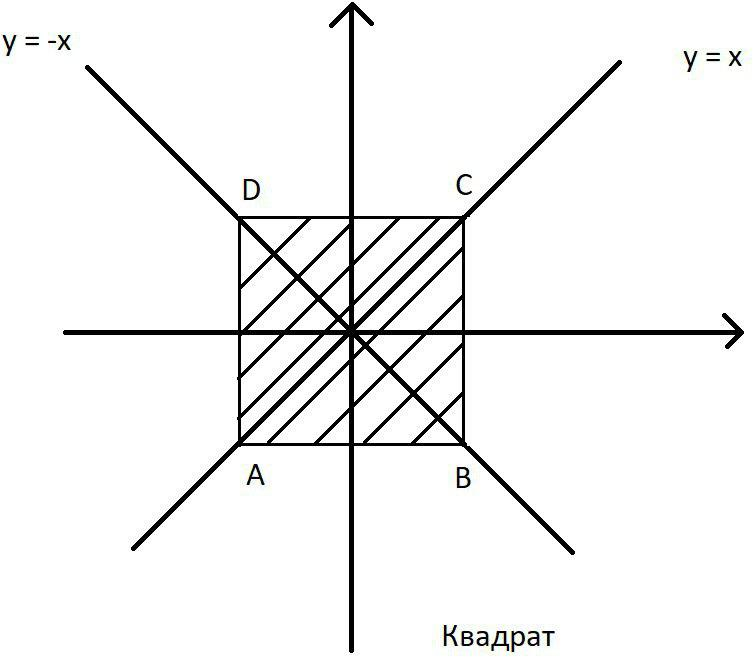
\includegraphics[scale = 0.7]{square.jpg}
		\end{center}
		
		\begin{enumerate}
		 \item $-x \le y \le x \implies x-y+x-y = 2x \le 2 \implies x \le 1$
         \item $-y \le x \le -y \implies \dots \implies y \le 1$
         \item $ \dots \implies x \ge -1$
         \item $ \dots \implies y \ge -1$
		\end{enumerate}
		
		Получаем, что $D$ является ограниченным и замкнутым, т.~е. компактом.
		
		Рассмотрим задачу на локальный экстремум на этом 
		компакте для функции $u = x^2 + y^2$:
		\begin{enumerate}
			\item[a)] Внутри $D$:
			
			$\begin{cases}
				u_{x}' = 2x = 0\\
				u_{y}' = 2y = 0\\
			\end{cases} \implies O(0; 0) \in D$~--- стационарная точка.
			
			\item[б)] На $\partial D$:
			
			\[\begin{array}{rl}
			x = -1, u = y^2 + 1 &\implies M_1(-1; 0)\\
			x = 1 &\implies M_2(1; 0)\\
			y = 1 &\implies M_3(0; 1)\\
			y = -1 &\implies M_4(0; -1)\\
			\end{array}\]
		\end{enumerate}
			
        К этим точкам необходимо добавить точки 
        недифференцируемости $\partial D$, т.~е. такие точки, где к $
        \partial D$ нет касательных.
        Этими точками будут $N_1(1; 1)$, $N_2(1; -1)$, 
        $N_3(-1; 1)$, $N_4(-1; -1)$.
        Далее вычислим значения функции во всех этих 
        точках:
        
        \[\begin{array}{rl}
        u(0; 0) &= 0 - \min \\
        u(M_{1, 2, 3, 4}) &= 1 \\
        u(N_{1, 2, 3, 4}) &= 2 - \max \\
        \end{array}\]
        
        \[\exists M = \max f(x) = 2\]
        \[\exists m = \min f(x) = 0\]
	\end{exmp}
\end{document}
